% Mirror: https://github.com/SIGma-UIUC/presentation-format
% --------------------------------------------------------------------
% This is a simple Beamer document that uses beamerthemesigma.sty
% Reading the comments should help you create a presentation even if
% you've never used Beamer before.
% --------------------------------------------------------------------

% Set our document class to Beamer
\documentclass[aspectratio=169]{beamer}

% Some packages for nice font encodings in the final PDF
\usepackage[utf8]{inputenc}
\usepackage[T1]{fontenc}

% From Jeff E
\usepackage{algo}

% Some more macros
\usepackage{sigmastyle}

% Citations
\usepackage{cite}

% To insert images
\usepackage{graphicx}

% Useful packages from the AMS
\usepackage{amsmath,amssymb,amsthm}

\usepackage{soul}

% Package for code highlighting
\usepackage{minted}
\setminted{linenos=true, breaklines=true, breakanywhere=true, style=default}
\usemintedstyle{monokai}

% Set a title
\title{Binary}
\subtitle{\cite[Chapter~7.2.1.1]{TAOCP4A}}

% Whoever worked on the presentation:
\author{Anakin}

% A date, if you'd like.
\date{}

% An institute name, if you're so inclined
% \institute{University of Illinois Urbana-Champaign}

% Use the SIGma theme for this Beamer presentation
\usetheme{sigma}
% --------------------------------------------------------------------

% Begin document
\begin{document}

% Beamer calls each slide a "frame", defined within the environment:
% \begin{frame}
%   <frame content here>
% \end{frame}

% This frame is just the title.
\begin{frame}
\titlepage
\end{frame}

% A frame with the table of contents.
% This frame's title is "Outline".
\begin{frame}{Outline}
  \tableofcontents
\end{frame}

\begin{frame}{What Are We Doing?}
    What is Combinatorics? \pause
    \begin{itemize}
        \item Existence
        \item Construction
        \item Enumeration
        \item Generation
        \item Optimization
    \end{itemize}
\end{frame}

\begin{frame}{What Are We Doing?}
    What is Combinatorics?
    \begin{itemize}
        \item \st{Existence}
        \item \st{Construction}
        \item \st{Enumeration}
        \item \textcolor{sigma@mainblue}{Generation} \textcolor{sigma@alertred}{(Our focus for today!)}
        \item \st{Optimization}
    \end{itemize}
\end{frame}


\section{Generating Tuples}
\frame{\sectionpage}

\begin{frame}{A Classic Problem}
    \begin{itemize}
        \item Suppose we wanted to \textcolor{sigma@mainblue}{generate} through all binary numbers from $\texttt{00000000} = 0$ through to $\underbrace{\texttt{11111111}}_{\textbf{8}\text{ 1s}} = 2^{\boldmath 8} - 1$ 
        \begin{itemize}
            \item Or more generally, $0$ through $2^n$ - 1 \pause
        \end{itemize}
        \item Equivalent to generate tuples $(a_n, \ldots, a_1)$ with $a_i \in \set{ \texttt{0}, \texttt{1}}$
        \begin{itemize}
            \item We write the tuple in this direction since we write numbers with bigger ``places'' to the left of smaller places \pause
        \end{itemize}
        \item We could even talk about other bases, like wanted to visit all base 10 numbers from $0$ through $10^n - 1$
    \end{itemize}
\end{frame}

\begin{frame}{The Obvious Algorithm (for $n = 8$)}
    \pause
    \begin{algo}
    \underline{\textsc{GenBinary}():}\+
    \\  For $a_1 \in \set{\texttt{0}, \texttt{1}}:$\+
    \\      For $a_2 \in \set{\texttt{0}, \texttt{1}}:$\+
    \\          For $a_3 \in \set{\texttt{0}, \texttt{1}}:$\+
    \\              For $a_4 \in \set{\texttt{0}, \texttt{1}}:$\+
    \\                  For $a_5 \in \set{\texttt{0}, \texttt{1}}:$\+
    \\                      For $a_6 \in \set{\texttt{0}, \texttt{1}}:$\+
    \\                          For $a_7 \in \set{\texttt{0}, \texttt{1}}:$\+
    \\                              For $a_8 \in \set{\texttt{0}, \texttt{1}}:$\+
    \\                                  \textsc{print}$(a_1 a_2 a_3 a_4 a_5 a_6 a_7 a_8)$
    \end{algo}
\end{frame}

\begin{frame}{We Can Do Better}
    \begin{itemize}
        \item What if we wanted to change our base from binary to base 10, or arbitrary base?
        \begin{itemize}
            \item Mixed base, also known as \textbf{mixed radix} \cite{TAOCP2}, numbers:
            \[
                \begin{bmatrix}
                            a_n, &a_{n - 1}, &\ldots, &a_1 \\
                            m_n, &m_{n - 1}, &\ldots, &m_1
                \end{bmatrix}
            \]
            \pause
            \item Examples for base 2 and time (0 index your days and months):
            \[
                \texttt{101001}_2 = \begin{bmatrix}
                            1, &0, &1, &0, &0, &1  \\
                            2, &2, &2, &2, &2, &2 
                \end{bmatrix},
            \]
            \[
                \text{2002-06-29 03:25:789} = \begin{bmatrix}
                            2002, &06, &29, &03, &25, &789 \\
                            \infty, &12, &30, &24, &60, &1000 
                \end{bmatrix}
            \]
            \pause
        \end{itemize}
    \end{itemize}
\end{frame}

\begin{frame}{Mixed-Radix Generation}
    \begin{nalgo}
    \underline{\textsc{Algorithm-M}(\emph{m}$[1..n]$):}
    \\\label{}  $a[i] \gets 0$ \textbf{for} $1 \leq i \leq n$ 
    \\\label{}  $a[n + 1] \gets 0$, $m[n + 1] \gets 2$ \Comment{\textbf{Exercise:} why do we need this?}
    \\\label{}  \textbf{while} \true:\+
    \\\label{}      \textsc{print}(\emph{a}$[n]$ $\cdots$ \emph{a}$[1]$)
    \\\label{}      $j \gets 1$
    \\\label{}      \textbf{while} $a[j] = m[j] - 1$\+
    \\\label{}          $a[j] \gets 0$
    \\\label{}          $j \gets j + 1$\-
    \\\label{}      \textbf{if} $j = n + 1$:\+
    \\\label{}          \textbf{return}\-
    \\\label{}      $a[j] \gets a[j] + 1$
    \end{nalgo}
    By setting $m[i] = 2$ for all $i$, we can print every binary number from $0$ to $2^n - 1$
\end{frame}

\begin{frame}{}
      \begin{center}
    {\color{sigma@mainblue} \LARGE Questions?}
  \end{center}
\end{frame}

\section{The Gray Code}
\frame{\sectionpage}

\begin{frame}{Becoming Lazier}
    \begin{itemize}
        \item Consider the fact that I am extremely lazy \pause
        \item If we are counting in binary and we count $\texttt{01111} \to \texttt{10000}$
        \begin{itemize}
            \item We have to change a whole \textbf{5} digits \textcolor{sigma@alertred}{The horror! The horror!}
            \item The inner \textbf{while} loop (Line 6) of \textsc{Algorithm-M} runs 5 times
        \end{itemize} \pause
        \item $n$ digits means $2^n$ numbers are generated, so $O\left(2^n\right)$ is our limit \pause
        \item For each digit, this inner \textbf{while} loop runs $O(n)$ times, resulting in total runtime $O\left(n 2^n \right)$ \pause
        \item Is there a way to avoid this and shave off a factor of $O(n)$?
    \end{itemize}
\end{frame}

\begin{frame}{Gray Binary Code}
    \begin{itemize}
        \item First appeared in a 1941 patent \#2307868 by George R. Stibitz
        \item Frank Gray mentioned the code in a 1947 patent \#2632058 
        \begin{itemize}
            \item As tradition, he gets the credit rather than the people before him
        \end{itemize} \pause
        \item He described a systematic way to generate binary where each successive number changes by exactly 1 digit for each step \pause
        \item Louis Gros published an anonymous note ``Th\'eorie du Baguenodier'' in Lyonnais, 1872, describing the Gray binary code in relation to solving an ancient Chinese puzzle \cite{baugenodier}.
        \begin{itemize}
            \item So in reality, he is the inventor
        \end{itemize}
    \end{itemize}
\end{frame}

% Doing this manually sucks
\begin{frame}{Generating the Gray Code}
    \begin{align*}
        \textit{Zero}& &\texttt{0}  \\
        \textit{One}&  &\texttt{1}  \\
    \end{align*}
\end{frame}

\begin{frame}{Generating the Gray Code}
    \begin{align*}
        \textit{Zero}& &\texttt{0}  \\
        \textit{One}&  &\texttt{1}  \\[-3\jot]
        &   &\underline{\hspace{20pt}}\\
                    &  &\texttt{1}  \\
                    &  &\texttt{0}  \\
    \end{align*}
\end{frame}

\begin{frame}{Generating the Gray Code}
    \begin{align*}
        \textit{Zero}& &\texttt{00}  \\
        \textit{One}&  &\texttt{01}  \\[-3\jot]
        &   &\underline{\hspace{20pt}}\\
                    &  &\texttt{11}  \\
                    &  &\texttt{10}  \\
    \end{align*}
\end{frame}

\begin{frame}{Generating the Gray Code}
    \begin{align*}
        \textit{Zero}& &\texttt{00}  \\
        \textit{One}&  &\texttt{01}  \\
        \textit{Three} &  &\texttt{11}  \\
        \textit{Two} &  &\texttt{10}  \\
    \end{align*}
\end{frame}

\begin{frame}{Generating the Gray Code}
    \begin{align*}
        \textit{Zero}& &\texttt{00}  \\
        \textit{One}&  &\texttt{01}  \\
        \textit{Three} &  &\texttt{11}  \\
        \textit{Two} &  &\texttt{10}  \\[-3\jot]
                    &   &\underline{\hspace{20pt}}\\
                        & &\texttt{10}  \\
                        &  &\texttt{11}  \\
                        &  &\texttt{01}  \\
                        &  &\texttt{00}  \\
    \end{align*}
\end{frame}

\begin{frame}{Generating the Gray Code}
    \begin{align*}
        \textit{Zero}& &\texttt{000}  \\
        \textit{One}&  &\texttt{001}  \\
        \textit{Three} &  &\texttt{011}  \\
        \textit{Two} &  &\texttt{010}  \\[-3\jot]
                    &   &\underline{\hspace{20pt}}\\
                        & &\texttt{110}  \\
                        &  &\texttt{111}  \\
                        &  &\texttt{101}  \\
                        &  &\texttt{100}  \\
    \end{align*}
\end{frame}

\begin{frame}{Generating the Gray Code}
    \begin{align*}
        \textit{Zero}& &\texttt{000}  \\
        \textit{One}&  &\texttt{001}  \\
        \textit{Three} &  &\texttt{011}  \\
        \textit{Two} &  &\texttt{010}  \\
        \textit{Six}    & &\texttt{110}  \\
        \textit{Seven}      &  &\texttt{111}  \\
        \textit{Five}    &  &\texttt{101}  \\
        \textit{Four}    &  &\texttt{100}  \\
    \end{align*}
\end{frame}

\begin{frame}{Generating the Gray Code}
    \begin{align*}
        \textit{Zero}& &\texttt{000}  \\
        \textit{One}&  &\texttt{00\textcolor{sigma@alertred}{\underline{1}}}  \\
        \textit{Three} &  &\texttt{0\textcolor{sigma@alertred}{\underline{1}}1}  \\
        \textit{Two} &  &\texttt{01\textcolor{sigma@alertred}{\underline{0}}}  \\
        \textit{Six}    & &\texttt{\textcolor{sigma@alertred}{\underline{1}}10}  \\
        \textit{Seven}      &  &\texttt{11\textcolor{sigma@alertred}{\underline{1}}}  \\
        \textit{Five}    &  &\texttt{1\textcolor{sigma@alertred}{\underline{0}}1}  \\
        \textit{Four}    &  &\texttt{10\textcolor{sigma@alertred}{\underline{0}}}  \\
    \end{align*}
\end{frame}

\begin{frame}{Recursive Definition}
    We can define the Gray Code recursively as follows
    \begin{equation}\label{rec_gray}
    \begin{split}
        \Gamma_0 &= \varepsilon \\
        \Gamma_{n + 1} &= \texttt{0} \cdot \Gamma_n,~ \texttt{1} \cdot \Gamma_n^R
    \end{split}
    \end{equation}
    where $\Gamma_n^R$ is $\Gamma_n$ and $0 \cdot \Gamma_n$ stands for appending 0 to every element in $\Gamma_n$ \pause
    
    \vspace{10pt}
    
    You can use this to prove that $gray(k) = k \oplus \left\lfloor \frac{k}{2} \right\rfloor$
    
    \vspace{60pt}    

    \textcolor{sigma@alertred}{\textbf{Exercise:}} Prove that $\Gamma_n$ generates all binary strings $0$ to $2^n - 1$
\end{frame}

\begin{frame}{Recursive Gray Code Generation}
    Here is some recursive code that makes use of the formula in Eq.~\ref{rec_gray}
    
    \begin{nalgo}
    \underline{\textsc{RecursiveGray}(n)}:
    \\\label{}  \textbf{if} $n = 0$:\+
    \\\label{}      \textbf{return} $[``\ "]$\-
    \\\label{}  $\Gamma_n \gets [~]$
    \\\label{}  $\Gamma_{n - 1} \gets \textsc{RecursiveGray}(n - 1)$
    \\\label{}  \textbf{for} \textit{num} $\in \Gamma_{n - 1}$:\+
    \\\label{}      $\Gamma_n$.\textsc{append}(\texttt{0} $\cdot$ \textit{num})\-
    \\\label{}  \textbf{for} \textit{num} $\in \Gamma_{n - 1}^R$:\+
    \\\label{}      $\Gamma_n$.\textsc{append}(\texttt{1} $\cdot$ \textit{num})\-
    \\\label{}  \textbf{return} $\Gamma_n$
    \end{nalgo} \pause
    
    Can we do this iteratively?
\end{frame}

\begin{frame}{Non-recursive Gray Code Generation}
    \begin{nalgo}
    \underline{\textsc{Algorithm-G}(\emph{n})}:\+
    \\\label{}  $a[i] \gets 0$ \textbf{for} $1 \leq i \leq n$
    \\\label{}  $a[0] \gets 0$ \Comment{\textbf{Exercise:} why do we need this?}
    \\\label{}  \textbf{while} \true:\+
    \\\label{}      \textsc{print}(\emph{a}$[n]$ $\cdots$ \emph{a}$[1]$)
    \\\label{}      $a[0] \gets 1 - a[0]$
    \\ \label{}      $j \gets$ \textbf{minimum} $j \geq 1$ such that $a[j - 1] = 1$
    \\\label{}      \textbf{if} $j = n + 1$:\+
    \\\label{}          \textbf{return}\-
    \\\label{}      $a[j] \gets 1 - a[j]$
    \end{nalgo} \pause
    We haven't really gotten rid of the inner \textbf{while} loop (the \textbf{minimum} on Line 6 is kind of a \textbf{while} loop). However, we only edit the array $a$ once per iteration of the outer loop.
\end{frame}

\begin{frame}{Loopless Non-recursive Gray Code Generation}
    \begin{nalgo}
    \underline{\textsc{Algorithm-L}(\emph{n})}:\+
    \\\label{}  $a[i] \gets 0$ \textbf{for} $1 \leq i \leq n$
    \\\label{}  $f[i] \gets i$ \textbf{for} $1 \leq i \leq n + 1$
    \\\label{}  \textbf{while} \true:\+
    \\\label{}      \textsc{print}(\emph{a}$[n]$ $\cdots$ \emph{a}$[1]$)
    \\\label{}      $j \gets f[1]$
    \\\label{}      $f[1] \gets 1$
    \\\label{}      \textbf{if} $j = n + 1$:\+
    \\\label{}          \textbf{return}\-
    \\\label{}      $a[j] \gets 1 - a[j]$
    \\\label{}      $f[j] \gets f[j + 1]$
    \\\label{}      $f[j + 1] \gets j + 1$
    \end{nalgo}
\end{frame}

\begin{frame}{What About Other Bases?}
    \begin{itemize}
        \item Can we do this change-one-digit-at-a-time thing with other bases? \pause
        \begin{itemize}
            \item Yes! We can even do it looplessly
        \end{itemize} \pause
        \item There are two somewhat natural ways of doing this: \emph{reflected}
    \end{itemize}
    \[
        000, 001, \ldots, 009, 019, 018, \ldots, 011, 010, 020, 021, 022, \ldots, 091, 090, 190, 191, \ldots
    \]\pause
    \begin{itemize}
        \item and \emph{modular}
    \end{itemize}
    \[
        000, 001, \ldots, 009, 019, 010, \ldots, 017, 018, 028, 029, 020, \ldots, 099, 090, 190, 191, \ldots
    \] \pause
    \begin{itemize}
        \item The following algorithm will generate the \emph{reflected} sequence.
        \begin{itemize}
            \item \textcolor{sigma@alertred}{\textbf{Exercise:}} Modify it to produce the modular sequence
        \end{itemize}
    \end{itemize}
\end{frame}

\begin{frame}{Loopless Reflected Mixed-Radix Gray Generation}
    \begin{nalgo}
    \underline{\textsc{Algorithm-H}(\emph{m}$[1..n]$):}
    \\\label{}  $a[i] \gets 0$ \textbf{for} $1 \leq i \leq n$
    \\\label{}  $f[i] \gets i$ \textbf{for} $1 \leq i \leq n + 1$
    \\\label{}  $d[i] \gets 1$ \textbf{for} $1 \leq i \leq n$ \Comment{directions}
    \\\label{}  \textbf{while} \true:\+
    \\\label{}      \textsc{print}(\emph{a}$[n]$ $\cdots$ \emph{a}$[1]$)
    \\\label{}      $j \gets f[1]$
    \\\label{}      $f[1] \gets 1$
    \\\label{}      \textbf{if} $j = n + 1$:\+
    \\\label{}          \textbf{return}\-
    \\\label{}      $a[j] \gets a[j] + d[j]$
    \\\label{}      \textbf{if} $a[j] = 0$ \textbf{or} $a[j] = m[j] - 1$:\+
    \\\label{}           $d[j] \gets -d[j]$ \Comment{change directions}
    \\\label{}          $f[j] \gets f[j + 1]$
    \\\label{}          $f[j + 1] \gets j + 1$
    \end{nalgo}
\end{frame}

\begin{frame}{}
      \begin{center}
    {\color{sigma@mainblue} \LARGE Questions?}
  \end{center}
\end{frame}

\section{Towers of Hanoi and A Chinese Ring Puzzle}
\frame{\sectionpage}

% Talk about Towers of Hanoi and the Chinese Ring Puzzle
\begin{frame}{Monks Moving Disks Until the World Ends}
    \begin{itemize}
        \item In 1883, French mathematician \'Edouard Lucas introduced his puzzle ``The Towers of Hanoi'' \pause
        \item Since then, this puzzle has had many mythical origin stories written about it
    \end{itemize}
    \begin{figure}
        \centering
        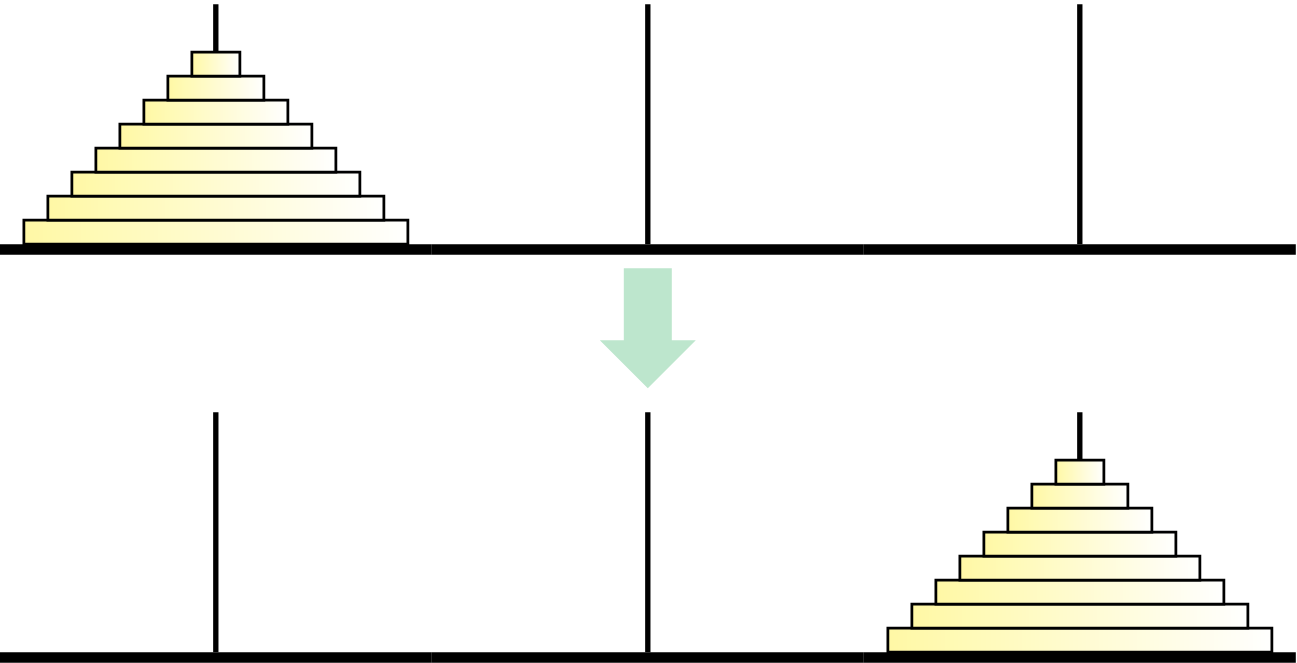
\includegraphics[scale=0.225]{images/hanoi.png}
        \caption{From \cite{book:algorithms}}
    \end{figure}
\end{frame}

\begin{frame}{Recursively Solving the Puzzle}
    \begin{figure}
        \centering
        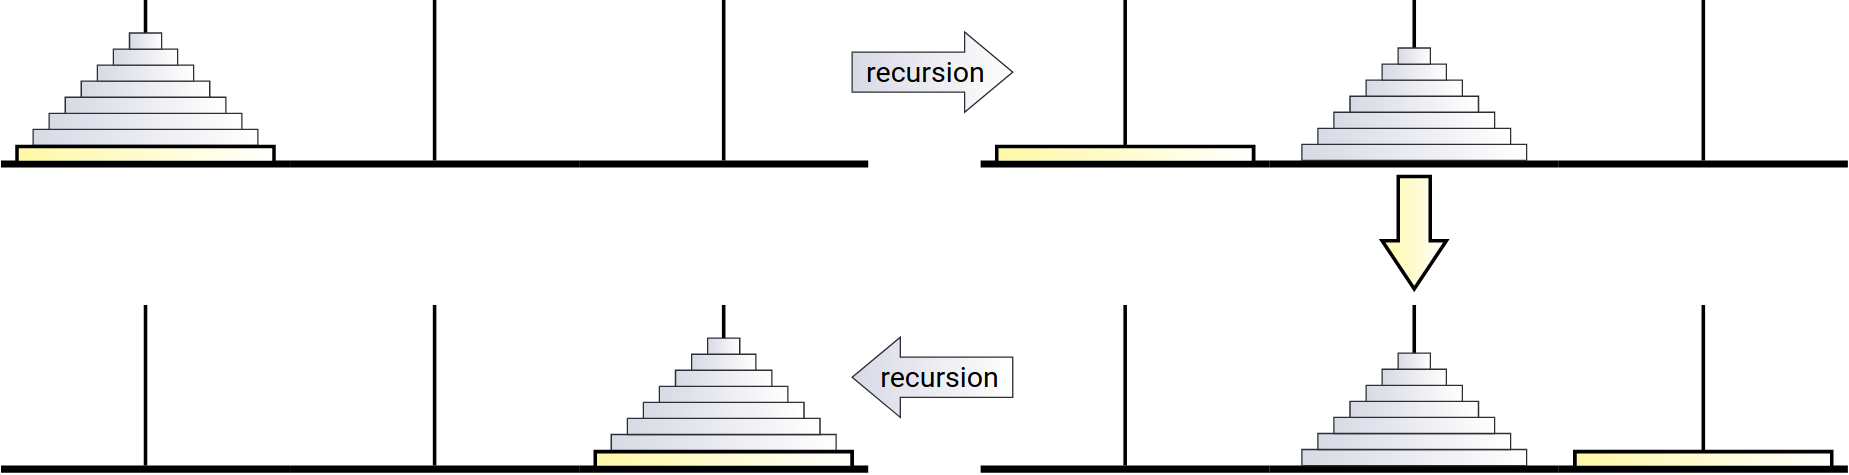
\includegraphics[scale=0.25]{images/recursive_hanoi.png}
        \caption{From \cite{book:algorithms}}
    \end{figure} \pause
    
    \begin{nalgo}
                \underline{\textsc{RecursiveHanoi}(n):}\+
    \\\label{}      Move the top $n - 1$ disks using \textsc{RecursiveHanoi}($n - 1$)
    \\\label{}      Move the $n$th disk
    \\\label{}      Move the top $n - 1$ disks using \textsc{RecursiveHanoi}($n - 1$)
    \end{nalgo}
\end{frame}

\begin{frame}{Iteratively Solving the Puzzle}
    \begin{itemize}
        \item The recursive solution takes $O\left( 2^n \right)$ time
        \item We can also solve the problem iteratively as follows
    \end{itemize}
    \begin{figure}
        \begin{nalgo}
            \underline{\textsc{IterativeHanoi}(n):}\+
        \\\label{}      \textbf{until} solved:\+
        \\\label{}          Move the small disk to the right
        \\\label{}          Make the only legal move not involving the small disk
        \end{nalgo}
        \caption{From \cite{sedgewick2003algorithms}}
    \end{figure}
\end{frame}

\begin{frame}{Solving the Puzzle using Binary}
    \begin{itemize}
        \item The following iterative algorithm uses \underline{binary} to iteratively solve the puzzle
        \item Suppose the smallest disk is disk $1$ and the largest disk is $n$
    \end{itemize}
    \begin{figure}
        \begin{nalgo}
            \underline{\textsc{BinaryHanoi}(n):}\+
        \\      $i \gets 0$
        \\      \textbf{while} $i < 2^n - 1$:\+
        \\          $i \gets i + 1$
        \\          $d \gets$ position of least significant $1$ in $\textsc{binary}(i)$
        \\          \textbf{if} $d = 1$:\+
        \\              Move the small disk to the right\-
        \\          \textbf{else}:\+
        \\              Move disk $d$ to the only legal position
        \end{nalgo}
        \caption{From \cite{3b1b_hanoi}}
    \end{figure}
\end{frame}

\begin{frame}{A Chinese Ring Puzzle}
    \begin{itemize}
        \item There is a similar puzzle, whose exact origin is unknown
        \begin{itemize}
            \item In Chinese, it is known as ``Jiu Lian Huan''
            \item In French, it is known as ``Baguenaudier''
        \end{itemize}
    \end{itemize}
    \begin{figure}
        \centering
        \scalebox{-1}[1]{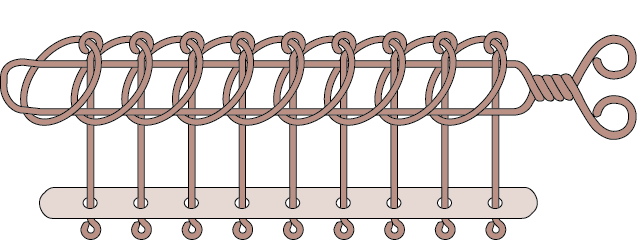
\includegraphics[scale=0.50]{images/baguenaudier_9.png}}
        \caption{From \cite{chinese_puzzle}}
    \end{figure}
\end{frame}

\begin{frame}{Allowed Moves}
    There are two legal moves we can make at each time
    \begin{itemize}
        \item We can remove and replace the rightmost ring at any time
        \item Any other ring can be removed or replaced as long as the following two conditions are met:
        \begin{itemize}
            \item The ring to its right is on the bar
            \item Every ring to the right of that is off the bar
        \end{itemize}
    \end{itemize}
    \begin{figure}
        \centering
        \scalebox{-1}[1]{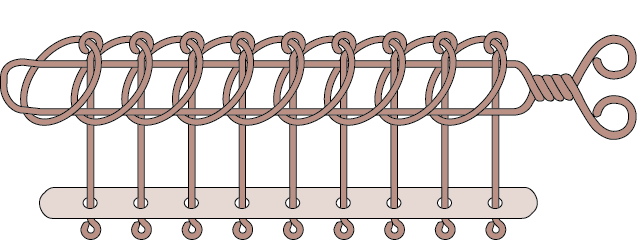
\includegraphics[scale=0.40]{images/baguenaudier_9.png}}
        \caption{From \cite{chinese_puzzle}}
    \end{figure}
\end{frame}

\begin{frame}{Solving the Puzzle}
    \begin{figure}
        \centering
        \scalebox{-1}[1]{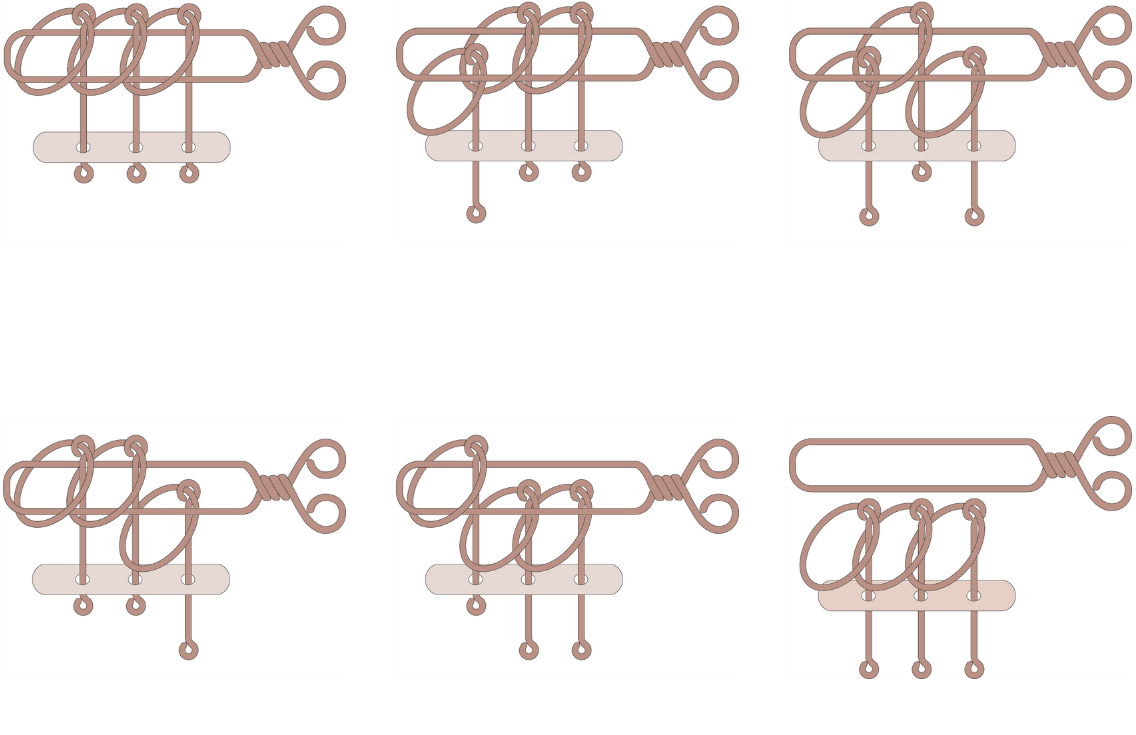
\includegraphics[scale=0.30]{images/baguenaudier_3.png}}
        \caption{From \cite{chinese_puzzle}}
    \end{figure}
\end{frame}

\begin{frame}{Algorithmically Solving the Puzzle}
    \begin{itemize}
        \item In his ``Th\'eorie du Baguenodier'' Louis Gros connected the Gray binary code to solving this ring puzzle
        \item Let us \textcolor{sigma@mainblue}{abstract} the puzzle into a series of binary digits
        \[
            \texttt{1111}
        \]
        \item The binary digit will be \texttt{1} if the ring is on and \texttt{0} otherwise
    \end{itemize}
\end{frame}

\begin{frame}{Algorithmically Solving the Puzzle}
    \vspace{-10pt}
    \begin{align*}
        \onslide<+->{&\texttt{1111}\\[0.01em]}
        \onslide<+->{&\texttt{1101}\\[0.01em]}
        \onslide<+->{&\texttt{1100}\\[0.01em]}
        \onslide<+->{&\texttt{0100}\\[0.01em]
        &\texttt{0101}\\[0.01em]
        &\texttt{0111}\\[0.01em]
        &\texttt{0110}\\[0.01em]
        &\texttt{0010}\\[0.01em]
        &\texttt{0011}\\[0.01em]
        &\texttt{0001}\\[0.01em]
        &\texttt{0000}}
    \end{align*} \pause
    This is Gray binary code starting from $\texttt{1111}$ and counting down to  $\texttt{0000}$
\end{frame}

\begin{frame}{}
      \begin{center}
    {\color{sigma@mainblue} \LARGE Questions?}
  \end{center}
\end{frame}

\font\eightss=cmssq8
\font\eightssi=cmssqi8
\newcommand\quoteAuthorDate[3]{\begingroup
  \baselineskip 10pt
  \parfillskip 0pt
  \interlinepenalty 10000 % not needed in example
  \leftskip 0pt plus 40pc minus \parindent
  \let\rm=\eightss
  \let\sl=\eightssi
  \everypar{\sl}#1\par
  \nobreak\smallskip
  \noindent\rm--- #2\unskip\enspace(#3)\par
  \endgroup}
% If someone can figure out how to horizontally center this and make the text bigger that'd be cool
\begin{frame}
    \begin{center}
        \item \quoteAuthorDate{It has been said that combinatorics is both the easiest and hardest field of mathematics. Easy since a lot of it requires no prerequisite knowledge. Hence a High School Student can do work in it. Hard because a lot of it requires no prerequisite knowledge. Hence you can’t easily apply continuous techniques.}{WILLIAM GASARCH}{\color{sigma@mainblue}\href{https://www.cs.umd.edu/~gasarch/open/pnpme.pdf}{2019}}
    \end{center}
\end{frame}

\begin{frame}{Bibliography}
    \bibliographystyle{alpha}
    {\tiny
    \bibliography{refs}
    }
\end{frame}

\end{document}